\chapter{Algorithms}
This chapter gives an introduction to different machine learning algorithms. It starts with two popular supervised learning algorithms, Support Vector Machines and K-Nearest Neighbors. Afterwards it explains how neural networks work. Finally some unsupervised techniques such as clustering and anomaly detection are discussed. 

\section{Support Vector Machines}
Support vector machines or SVMs is a supervised learning algorithm which offers an alternative view on logistic regression. Support vector machines try to find a model which devides the 2 classes exactly with the same amount of margin on either side as shown in Figure~\ref{fig:svm}. Samples on the margin are called the support vectors.
\begin{figure}[H]
\centering
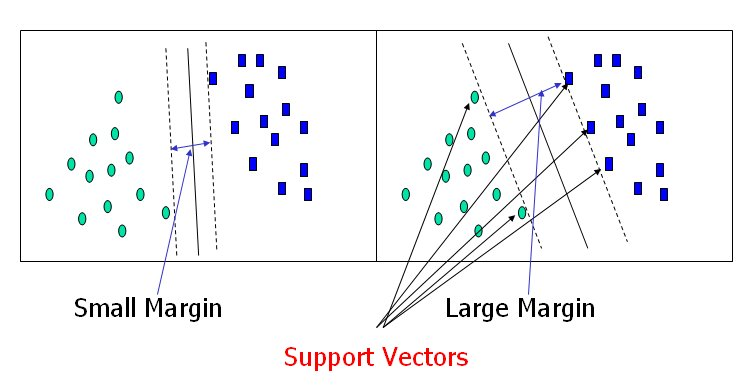
\includegraphics[width=\textwidth]{Figures/svm}
\decoRule
\caption[Support Vector Machines]{Support vector machines with their support vectors. \cite{svm}}
\label{fig:svm}
\end{figure}
\noindent In order to adapt Support Vector Machines to be able to fit non-lineair classifiers, some adjustments need to be done. This can be done with kernels. A kernel is a similarity function. The function compares two inputs and computes their similarity. Normally features are extracted from data and then fed into a machine learning algorithm. Kernels offer an alternative. The kernel should be a function to compare input data. The kernel, along with labeled data is then used to construct features. Using no kernel is called a lineair kernel. The basic type of kernel algorithms are called Gaussian kernels. The formula for Gaussian kernels is:
\begin{align}
K(x,y) = \exp{(\dfrac{-||x-y||^2}{2\sigma^2})}
\end{align}

\section{K-Nearest Neighbors}
The K-Nearest Neighbors or KNN algorithm is an algorithm which computes the classification by looking at the classes of the K-Nearest neighbors of the inputted data. The K-Nearest Neighbors is an Instance-based algorithm. \cite{mlcat} The chosen class is the class most common among its K-Nearest neighbors, this can be seen in Figure~\ref{fig:knn}. K is typically a small number. When K is equal to 1, the assigned class is the same as the class of the closest sample. \\\\
When training the algorithm, the input data and classes are stored. There are mutliple methods to compute the distance between data. Euclidean distance can be used for continous data. For discrete variables another metric can be used, such as the overlap metric or Hamming distance.\\\\
A major drawback of the KNN algorithm is the weakness to skewed data. Since the class is chosen based on the most popular nearest class, these popular classes may dominate the prediction. This can be overcome by taking the distance between the input data and the neighbors into account.
\begin{figure}[H]
\centering
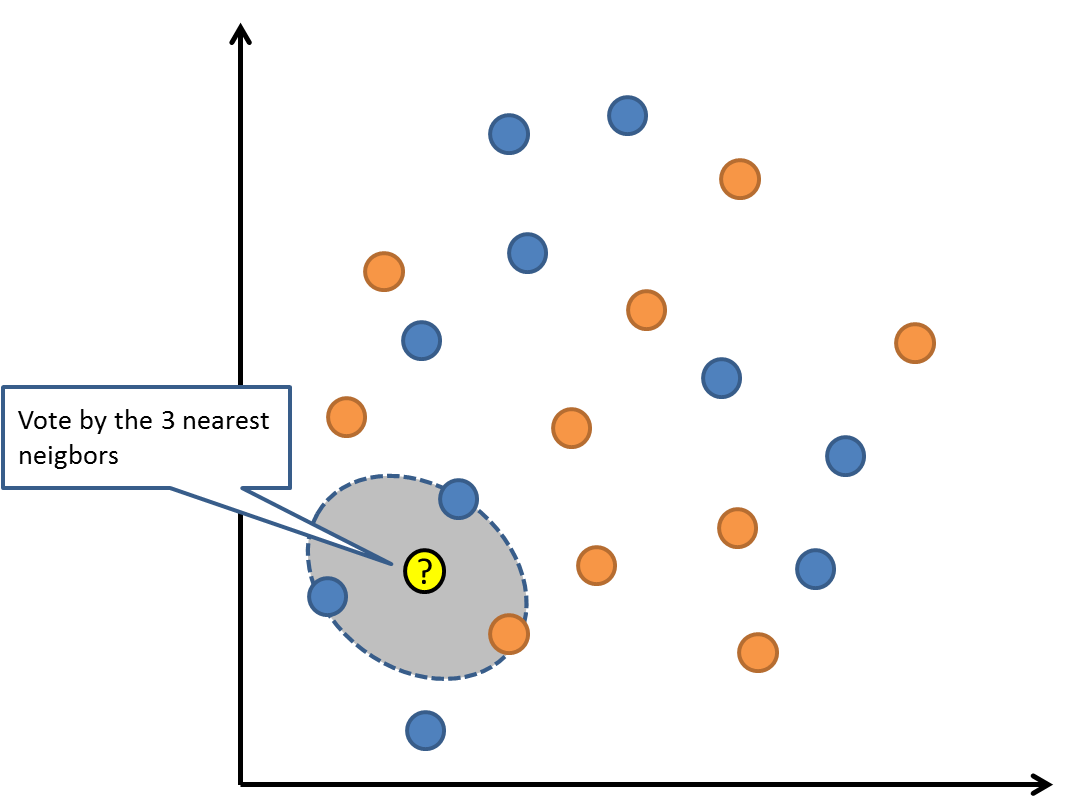
\includegraphics[width=0.8\textwidth]{Figures/knn}
\decoRule
\caption[K-Nearest Neighbors]{K-Nearest Neighbors. \cite{knn}}
\label{fig:knn}
\end{figure}

\section{Clustering}
Clustering is a machine learning concept using unsupervised learning. Unsupervised learning does not have labels with the training set. An unsupervised machine learning algorithm tries to find structure within the given training set. Clustering is the first type of unsupervised learning. It tries to cluster the training samples into different clusters.

\subsection{K-means Algorithm}
The K-means algorithm is a simple clustering algorithm. K is the number of clusters that is going to be used. The algorithm first randomly places the K clusters in the space (from the training set). This can be done by randomly chosing K training samples. Then it repeats the following steps until the cluster centers remain stationary. it iterates over all training samples, and assigns them to the closest cluster. Next the cluster centers are moved to the center of the total cluster. \\\\
The cluster centroids will be addressed using the symbol $\mu$ with $\mu_k$ the cluster centroid of cluster k. $c^{(i)}$ is the index of the cluster to which training sample  $x^{(i)}$ has been assigned. $\mu_{c^{(i)}}$ is the cluster centroid to which training sample $x^{(i)}$ has been assigned. The cost function can be described as:
\begin{align}
J(c, \mu) = \dfrac{1}{m} \sum\limits_{i=1}^m(|| x^{(i)} - \mu^{(i)}||)^2
\end{align}
The final clusters that are found by K-means are dependent on the random placement of the K clusters in the beginning. It could lead to suboptimal clustering. This can be fixed by running K-means a number of times and after each iteration check the value of the cost function to find the most efficient run of K-means. \\\\
There is a similar problem with determining the amount of clusters. The same method could be used to determine the correct number of clusters. However, manually determining the number of clusters could be more time efficient.
\section{Neural networks}
Neural networks are a useful alternative to logistic regression if the amount of features becomes too large. The origin of neural networks are algorithms which try to mimic the brain. There is a hypothesis, the "one learning algorithm" hypothesis, that shows that the brain can learn very different things, such as sound, touch, etc. by using a single algorithm. \\\\
A neural network is created of neurons, which are called a logistic unit. Each neuron receives input wires, and has an output wire, which computes a value using the sigmoid (logistic) hypothesis, the activation function. A neural network is a group of "neurons" that are connected together. This can be grouped into a layered approach as seen in Figure~\ref{fig:neuralnetwork}. The first layer is called the input layer, the final layer is called the output layer which outputs a $H_\theta(x)$ which is class. All layers inbetween these layers are called hidden layers.
\begin{figure}[H]
\centering
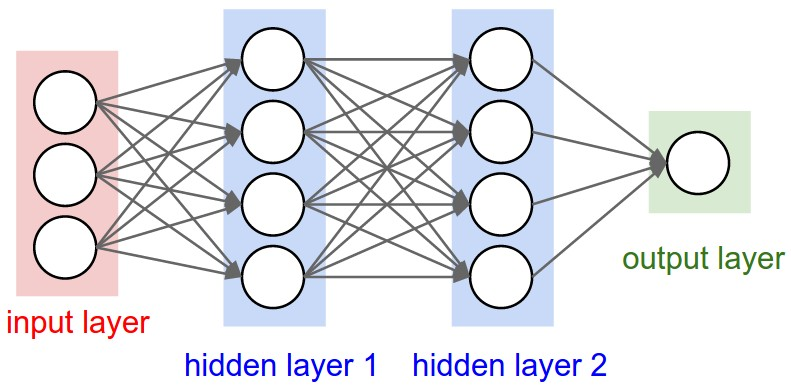
\includegraphics[width=1\textwidth]{Figures/neuralnet}
\decoRule
\caption[Neural network]{A neural network showing the different layers.\cite{neuralnetwork}}
\label{fig:neuralnetwork}
\end{figure}
\noindent Each logistic unit is denoted by $a_i^j$. $j$ is the layer and $i$ is the position in that layer. $\theta^j$ is a matrix of weights or parameters controlling function mapping from layer $j$ to layer $j+1$. $s_l$ is the number of units within a layer. The number of layers is denoted by $L$.\\\\The neural network works similar to logistic regression, except that it performs logistic regression from layer to layer. The parameters $\theta_j$ required are learned by itself. The architecture of a neural network refers to the way the units are connected to eachother. Neural networks can be used for multi-class classification. Hereby there are mutliple units in the output layer and each unit represents a different class. $K$ will denote the amount of output units.
\begin{figure}[H]
\centering
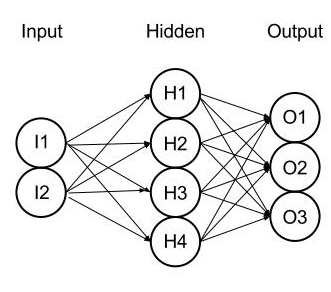
\includegraphics[width=0.7\textwidth]{Figures/neuralnetmulti}
\decoRule
\caption[Neural network with multi-class classification]{A neural network capable of multi-class classification. \cite{neuralnetworkmult}}
\label{fig:neuralnetworkmult}
\end{figure}
\noindent Data flows using the principle of forward propagation. The data passes through the first layers, move to the second layers and so on, until it arrives at the final layer. Mathematically this can be described as: 
\begin{align*}
a^{(1)} = x\\
z^{(2)} = \theta^{(1)}*a^{(1)}\\
a^{(1)} = g(z^{(2)})
\end{align*}
\subsection{Cost function and backpropagation}
The cost function for neural networks is a generalisation of the cost function for logistic regression. The cost function accounts for the different layers, units and the number of output units. To minimize the cost function, the same methods such as gradient descent can be used. However, the problem is how to compute the partial derivative of the cost function. Using backpropagation, it is possible to compute this. \\\\
The resulting class is known in the final layer. From here, the algorithm can find the error. $\delta_j^l$ will be the symbol used for the error of node $j$ in layer $l$. For an example with 4 layers:
\begin{align}
\delta_j^{(4)} = a_j^{(4)} - y_j\\
\delta^{(3)} = (\theta^{(3)})^T\delta^{(4)} * g'(z^{(3)})
\end{align}
The algorithm starts by setting a parameter $\Delta_{ij}^{(l)}$ to 0 for all $i$, $j$, $l$. Then, it iterates from $i=0$ to $m$, with $m$ the number of training samples. Each iteration, $a^{(1)}$ is set to $x^{(i)}$. Forward propagation is computed for $a^{(l)}$ for all $l = 2,3,..., L$. Using $y^{(i)}$, $\delta^{(L)}$ can be computed. Then the different $\delta^{(L-1)}$ to $\delta^{(2)}$ are computed. Finally, $\Delta_{ij}^{(l)}$ is incremented by $a_j^{(l)}\delta^{(l+2)}$ for each $l$. After the iteration is done, the final value for the partial derivative can be calculated: $\dfrac{\partial}{\partial \theta_ij^{(l)}} J(\theta)$. This can be done by dividing $\Delta_{ij}^{(l)}$ by the amount of training samples and adding $\lambda\theta_ij^{(i)}$. 
\subsection{Using a neural network}
A neural network should have as many input units as the dimension of features. The number of output units is equal to the number of classes. Default, there should be either 1 hidden layer or if there are more, all layers should have the same number of hidden units. The neural network should be trained by first assigning random weights to the values of $\theta$. Afterwards, forward propagation should be used to get $H_\theta(x^{(i)}$. Next the cost function should be computed. Backwards propagation is used to compute the partial derivatives. The result of backwards propagation can be checked by numerical methods to compute the gradient. Finally gradient descent or other advanced optimization methods with backpropagation should be used to try to minimize the cost function as a function to the parameters $\theta$.
\section{Dimensionality reduction}
Dimensionality reduction is the process of reducing the amount of features used in machine learning algorithms. This can be used to increase the accuracy and the performace of machine learning algorithms. One form is to do data compression. For example, transform 3D data into 2D data and eliminating a feature or dimension. It can also be used to reduce dimensions to be able to efficiently visualise data.

\subsection{Principle Component Analysis}
Principle Component Analysis is a way to do dimensionality reduction. The algorithm is formed as a minimalisation problem. When given N-dimensional data and N-1 dimensional data is prefered. The algorithm tries to find the correct N-1 dimensional value so that the projection is the closest to the original data. \\\\
Before this algorithm should be run, the features of the data should be scaled, so all features are on a similar scale. This can be done by using mean normalization. In order to reduce the dimension from $n$ to $k$ the covariance matrix should be computed:
\begin{align}
\Sigma = \dfrac{1}{m}\sum\limits_{i=1}^n((x^{(i)}) (x^{(i)})^T)
\end{align}
From this matrix, the eigenvectors need to be computed using singular value decomposition. From these values, only the first $k$ values are going to be used and be multiplied with the training data.\\\\
PCA can be used to speed up the time it takes for other learning algorithms to learn. By using PCA, the amount of features or the amount of training samples is reduced which reduces the running time of the training, but the compressed data still retains the same information as the uncompressed data.

\section{Anomaly detection}
Anomaly detection is also a form of unsupervised learning. The algorithm learns what normal behaviour looks like through the training set and then tries to predict if a given input data belongs to the normal behaviour or is abnormal for any reason.
\begin{figure}[H]
\centering
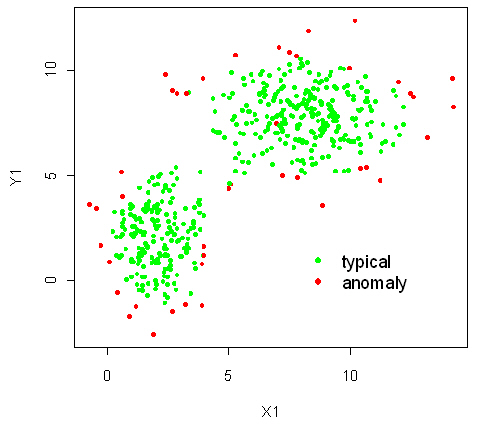
\includegraphics[width=0.8\textwidth]{Figures/anomaly}
\decoRule
\caption[Anomaly detection]{Anomaly detection. \cite{anomaly-fig}}
\label{fig:anomalydetection}
\end{figure}
\noindent Anomaly detection algorithms make heavy use of (Gaussian) Normal distribution:
\begin{align}
x \sim N(\mu, \sigma^2)
\end{align}
Hereby is $\mu$ the mean parameter and $\sigma$ is the standard deviation. Now the probability of $x$ being an anomaly can be calculated as:
\begin{align}
p(x) = \prod_{j=1}^n( \dfrac{1}{\sqrt{2\pi}\sigma_j} exp(- \dfrac{(x_j - \mu_j)^2}{2\sigma_j^2}) )
\end{align}

\section{Other algorithms}
There are also other, more specific and advanced categories of machine learning algorithms. There are decision tree algorithms, for example, Classification and Regression Tree (CART), Conditional Decision Trees, etc. There are Bayesian Algorithms which explicitly apply Bayes’ Theorem for problems such as classification and regression. These algorithms include Naive Bayes, Gaussian Naive Bayes, Multinomial Naive Bayes, etc. \cite{mlcat} \\\\
Association Rule Learning Algorithms are methods that extract rules that best explain observed relationships between variables in data. Apriori algorithm and Eclat algorithm are examples of such algorithms. Deep Learning Algorithms are a modern modification to Artificial Neural Networks that exploit abundant cheap computation. Deep learning networks are very deep and complex neural networks. Deep Boltzmann Machine (DBM), Deep Belief Networks (DBN) and Convolutional Neural Network (CNN) are examples of deap learning algorithms.  \cite{mlcat}\\\\
Ensemble Algorithms such as Bootstrapped Aggregation (Bagging) are models that combine multiple weaker models and try to combine the predictions made by these models. Yet there are still many more algorithms.  \cite{mlcat}\\\\
A lot of algorithms are specifically constructed for a specific sub-field of machine learning, for example computer vision, natural language processing, etc. Even within the categories of algorithms that were discussed, regression, regularization, instance-based, clustering, neural networks and dimensionality reduction, there are a lot of different variants. However, these are considered to be to advanced and outside the scope of this thesis. 
